\chapter{Background and Literature Review}
\label{ch:motivation}

There is a vast body of algorithms for Sparse Matrix Multiplication (SpMM),
as well as many different storage formats for converting sparse matrices into
representations that can be operated on efficiently. This chapter provides
the information needed to understand the context and design decisions taken
throughout this project, alongside the goals that were set out at the start.
If any of the material that follows is unfamiliar, a more elementary
overview of SpMM and the CSR format is given in
Appendix~\ref{app:spmm-background}, and further reading can be pursued
through the references cited in each section.
\section{SpMM in Modern Workloads}

The motivation for a dedicated SpMM accelerator is made concrete by the
sparsity levels that real workloads exhibit. Figure~\ref{fig:sparsity-levels}
summarises representative density ranges across four workload classes: in
each case, the fraction of nonzero entries is small enough that storing and
operating on the matrix in dense form would be wasteful by one to five
orders of magnitude.

\begin{figure}[htbp]
  \centering
  \hspace*{-1.5cm}%
  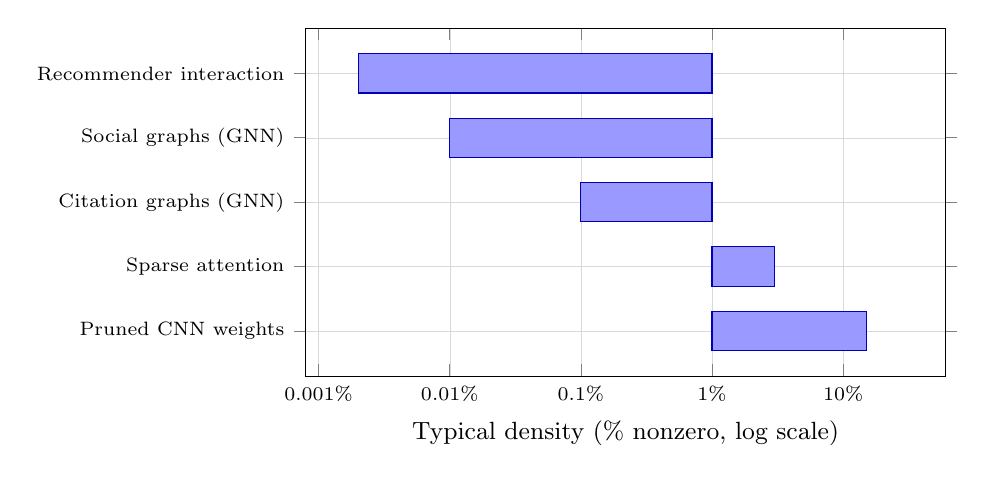
\begin{tikzpicture}
    \begin{axis}[
      width=0.8\linewidth, height=6cm,
      xbar,
      xmode=log,
      log basis x=10,
      xmin=0.0008, xmax=60,
      xlabel={Typical density (\% nonzero, log scale)},
      ytick={1,2,3,4,5},
      yticklabels={
        {Recommender interaction},
        {Social graphs (GNN)},
        {Citation graphs (GNN)},
        {Sparse attention},
        {Pruned CNN weights}},
      y dir=reverse,
      ymin=0.3, ymax=5.7,
      bar width=5mm,
      xtick={0.001,0.01,0.1,1,10},
      xticklabels={0.001\%,0.01\%,0.1\%,1\%,10\%},
      tick label style={font=\scriptsize},
      label style={font=\small},
      grid=major,
      major grid style={line width=.1pt, draw=gray!30},
    ]
      \addplot[fill=blue!40, draw=blue!70!black] coordinates {
        (0.002, 1)
        (0.01,  2)
        (0.1,   3)
        (3,     4)
        (15,    5)
      };
    \end{axis}
  \end{tikzpicture}
  \caption{Representative density ranges for matrices encountered in four
           classes of modern workload. Social and citation graphs in GNN
           benchmarks such as \texttt{ogbn-arxiv} and \texttt{Reddit} typically
           have densities below 0.1\%~\citep{graphsage2017}; large-scale
           recommender interaction matrices are often two orders of magnitude
           sparser still~\citep{covington2016youtube}. Pruned CNNs sit at the
           other end of the range, retaining 10--20\% of their weights after
           aggressive pruning~\citep{han2016eie}. In every case, an SpMM
           execution model that iterates only over the nonzeros avoids between
           90\% and $>99.99$\% of the arithmetic that a dense multiply would
           perform.}
  \label{fig:sparsity-levels}
\end{figure}

\subsection{Graph Neural Networks}

Graph neural networks (GNNs) represent the most rapidly growing class of workloads
in which SpMM appears as a first-class primitive. In message-passing GNNs such as
GraphSAGE~\citep{graphsage2017} and Graph Attention Networks~\citep{gat2018}, each
layer computes
\[
  H^{(l+1)} = \sigma\!\left( \hat{A} \, H^{(l)} \, W^{(l)} \right),
\]
where $\hat{A}$ is the normalised sparse adjacency matrix of the input graph,
$H^{(l)}$ is the dense feature matrix at layer $l$, and $W^{(l)}$ is a dense
weight matrix. The product $\hat{A} \, H^{(l)}$ is a sparse--dense matrix
multiply: $\hat{A}$ is sparse (real-world social and citation graphs can have
densities below 0.01\%), while $H^{(l)}$ is dense with feature dimension
typically 64--2048. This SpMM step dominates GNN inference time in practice,
particularly for large graph datasets where $\hat{A}$ has billions of edges.

\subsection{Recommender Systems and Sparse Embedding Lookup}

Industrial recommender systems such as the YouTube recommendation engine
\citep{covington2016youtube} maintain item--feature embedding tables that can
reach hundreds of millions of rows. The forward pass performs sparse embedding
lookups that reduce to a row-gather SpMM on the interaction matrix. Because the
interaction patterns are highly sparse and the embedding matrices are dense, the
memory-access pattern is irregular and the workload is inherently SpMM-shaped.

\subsection{Scientific Computing}

In finite-element and finite-difference simulation, sparse matrices arise from
the discretisation of differential operators on computational meshes. The
structure of the sparse factor is dictated by the mesh topology, which is
problem-dependent and generally irregular. SpMM in this setting appears in
multivector iterative solvers such as block GMRES and Lanczos methods, where
each Krylov iteration applies the sparse system matrix to a block of several
dense vectors simultaneously.

\subsection{Compressed and Pruned Neural Networks}

Weight pruning removes less-significant connections from a dense neural network,
increasing the proportion of zero weights and making weight matrices suitable for
sparse representation. Han et al.~\citep{han2016eie} demonstrated that networks
pruned to 80--90\% sparsity can be represented and executed in compressed form
with significant reductions in energy and storage. When combined with INT8
quantisation, as in the EIE design, SpMM on the compressed weight matrix becomes
the dominant kernel. The same principle applies to attention heads in transformers
that adopt sparse attention patterns.

\section{Why Sparsity Changes the Design Problem}

\subsection{The FLOP-to-Bandwidth Mismatch}

Dense matrix multiplication exhibits high operational intensity: for an
$M \times K \times N$ dense GEMM, the ratio of FLOPs to bytes loaded is
$O(N)$ when data is reused across the $N$ output columns. Sparse matrix
multiplication loses this reuse structure. For a CSR SpMM with $\text{NNZ}$
nonzeros, the number of useful MACs per byte of CSR index data fetched is
\[
  \text{OI} = \frac{2 \cdot \text{NNZ} \cdot N}
                   {\text{NNZ} \cdot (4 + 4) + (M + 1) \cdot 4 + \text{NNZ} \cdot 4 \cdot N},
\]
where the denominator accounts for \texttt{colidx} (4 bytes per entry),
\texttt{values} (4 bytes per entry), \texttt{rowptr} (4 bytes per pointer), and
the dense $B$ segment reads (4 bytes per column per nonzero). For small $N$ and
low density, the operational intensity is significantly below the roofline knee
of typical on-chip BRAM systems~\citep{williams2009roofline}, confirming that
SpMM is memory-bandwidth-limited rather than compute-limited on most platforms.

\subsection{Irregular Access and Control-Flow Overhead}

Beyond raw bandwidth, SpMM imposes control overhead that dense accelerators are
not designed to handle. For each nonzero $a_{ij}$, the hardware must:
\begin{enumerate}
  \item read the column index $j$ from \texttt{colidx};
  \item compute the address of the relevant row of $B$ as $\text{B\_base} + j \cdot N$;
  \item read the $N$ values of $B[j, :]$; and
  \item accumulate $a_{ij} \cdot B[j, n]$ into $C[i, n]$ for each column $n$.
\end{enumerate}
Steps (1) and (2) involve indirection: the address of the $B$ row is not known
until the column index has been loaded. This pointer-chasing pattern breaks
prefetching and creates a data-dependent dependency chain that is difficult for
out-of-order processors to hide. On a simple in-order core such as PicoRV32,
each nonzero must be handled sequentially, making the control overhead dominate
the total execution time. Figure~\ref{fig:access-pattern} contrasts the
predictable stride of a dense traversal with the indirect, data-dependent
address sequence that CSR SpMM produces.

\begin{figure}[htbp]
  \centering
  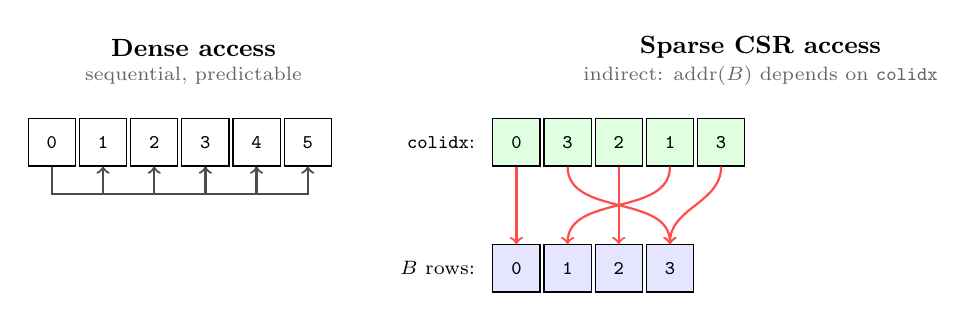
\begin{tikzpicture}[
      every node/.style={font=\small},
      cell/.style={draw, minimum width=6mm, minimum height=6mm, inner sep=0pt,
                   font=\scriptsize\ttfamily, anchor=center},
      acell/.style={draw, minimum width=6mm, minimum height=6mm, inner sep=0pt,
                    font=\scriptsize\ttfamily, fill=green!12},
      bcell/.style={draw, minimum width=6mm, minimum height=6mm, inner sep=0pt,
                    font=\scriptsize\ttfamily, fill=blue!10},
    ]
    % --- LEFT: dense access ---
    \node[font=\small\bfseries] at (1.8,2.6) {Dense access};
    \node[font=\scriptsize, text=black!60] at (1.8,2.25) {sequential, predictable};
    \foreach \i in {0,1,2,3,4,5} {
      \node[cell] (d\i) at (\i*0.65, 1.4) {\i};
    }
    \draw[->, thick, black!70] (d0.south) -- ++(0,-0.35) -| (d1.south);
    \draw[->, thick, black!70] (d1.south) -- ++(0,-0.35) -| (d2.south);
    \draw[->, thick, black!70] (d2.south) -- ++(0,-0.35) -| (d3.south);
    \draw[->, thick, black!70] (d3.south) -- ++(0,-0.35) -| (d4.south);
    \draw[->, thick, black!70] (d4.south) -- ++(0,-0.35) -| (d5.south);

    % --- RIGHT: sparse access ---
    \node[font=\small\bfseries] at (9.0,2.6) {Sparse CSR access};
    \node[font=\scriptsize, text=black!60] at (9.0,2.25)
      {indirect: addr$(B)$ depends on \texttt{colidx}};

    % colidx row
    \node[font=\scriptsize, anchor=east] at (5.5,1.4) {\texttt{colidx}:};
    \foreach \val [count=\i from 0] in {0,3,2,1,3} {
      \node[acell] (ci\i) at (5.9+\i*0.65, 1.4) {\val};
    }

    % B rows (destination) laid out as indexed rows
    \node[font=\scriptsize, anchor=east] at (5.5,-0.2) {$B$ rows:};
    \foreach \row in {0,1,2,3} {
      \node[bcell] (B\row) at (5.9+\row*0.65, -0.2) {\row};
    }

    % indirect pointer arrows: ci0 -> B0, ci1 -> B3, ci2 -> B2, ci3 -> B1, ci4 -> B3
    \draw[->, thick, red!70, out=-90, in=90] (ci0.south) to (B0.north);
    \draw[->, thick, red!70, out=-90, in=90] (ci1.south) to (B3.north);
    \draw[->, thick, red!70, out=-90, in=90] (ci2.south) to (B2.north);
    \draw[->, thick, red!70, out=-90, in=90] (ci3.south) to (B1.north);
    \draw[->, thick, red!70, out=-90, in=90] (ci4.south) to (B3.north);
  \end{tikzpicture}
  \caption{Memory access patterns in dense versus sparse CSR traversal. Dense
           access strides sequentially through contiguous addresses, so a
           prefetcher can fetch ahead. CSR access loads a column index from
           \texttt{colidx} first, then uses that value as an indirect pointer
           into $B$; the next address cannot be known until the previous load
           completes, which breaks prefetching and produces data-dependent
           cache misses.}
  \label{fig:access-pattern}
\end{figure}

\section{Sparse Matrix Storage Formats}

Several sparse matrix storage formats have been proposed; the choice of format
strongly affects the hardware control structure. Table~\ref{tab:sparse-formats}
summarises the most relevant formats and their suitability for hardware
acceleration.

\begin{table}[htbp]
  \centering
  \small
  \setlength{\tabcolsep}{2pt}
  \begin{tabular}{llp{4.0cm}p{3.5cm}}
  \toprule
  Format & Acronym & Description & Hardware suitability \\
  \midrule
  Coordinate list & COO &
    Stores (row, col, val) triplets unsorted or sorted by row.
    Simple to generate; requires sorting for efficient row-wise access. &
    High overhead per nonzero; poor for row-streaming hardware. \\[4pt]
  Compressed Sparse Row & CSR &
    Three arrays: \texttt{rowptr} ($M{+}1$ entries), \texttt{colidx} (NNZ),
    \texttt{values} (NNZ). Row bounds are contiguous. &
    Excellent for row-wise traversal; natural hardware FSM mapping. \\[4pt]
  ELLPACK & ELL &
    Pads each row to the maximum NNZ per row; stores in column-major order. &
    Good for regular sparsity; wastes storage and bandwidth when rows vary widely. \\[4pt]
  Block Compressed Sparse Row & BSR &
    Groups nonzeros into dense $r \times c$ blocks stored in CSR form. &
    High throughput on block-sparse matrices; unsuitable for unstructured sparsity. \\[4pt]
  Compressed Sparse Column & CSC &
    Transpose of CSR; columns are compressed. &
    Natural for column-wise access patterns; awkward for row-oriented output. \\
  \bottomrule
  \end{tabular}
  \caption{Comparison of common sparse matrix storage formats and their suitability
           for hardware acceleration.}
  \label{tab:sparse-formats}
\end{table}

\subsection{Why CSR Was Chosen}

Figure~\ref{fig:csr-layout} shows the CSR encoding of a small $4 \times 4$
sparse matrix. The three arrays \texttt{rowptr}, \texttt{colidx}, and
\texttt{values} together record exactly which nonzeros exist and where, with
no storage spent on the zero entries.

\begin{figure}[htbp]
  \centering
  \begin{tikzpicture}[
      every node/.style={font=\small},
      mcell/.style={draw, minimum size=7mm, inner sep=0pt, anchor=center},
      acell/.style={draw, minimum width=7mm, minimum height=6mm, inner sep=0pt,
                    font=\scriptsize\ttfamily},
    ]
    % --- Matrix A ---
    \node[font=\small] at (-0.2,3) {Matrix $A$};
    \matrix (A) [matrix of nodes,
                 nodes={mcell},
                 column sep=-\pgflinewidth,
                 row sep=-\pgflinewidth,
                 nodes in empty cells] at (0,1) {
      3 & 0 & 0 & 7 \\
      0 & 0 & 2 & 0 \\
      0 & 5 & 0 & 0 \\
      0 & 0 & 0 & 1 \\
    };

    % --- rowptr ---
    \node[font=\small, anchor=west] at (3.6,2.5) {\texttt{rowptr}};
    \foreach \val [count=\i from 0] in {0,2,3,4,5} {
      \node[acell, fill=blue!10] (rp\i) at (4.2+\i*0.75, 2.05) {\val};
    }

    % --- colidx ---
    \node[font=\small, anchor=west] at (3.6,1.3) {\texttt{colidx}};
    \foreach \val [count=\i from 0] in {0,3,2,1,3} {
      \node[acell, fill=green!12] (ci\i) at (4.2+\i*0.75, 0.85) {\val};
    }

    % --- values ---
    \node[font=\small, anchor=west] at (3.6,0.1) {\texttt{values}};
    \foreach \val [count=\i from 0] in {3,7,2,5,1} {
      \node[acell, fill=orange!15] (vl\i) at (4.2+\i*0.75, -0.35) {\val};
    }

    % --- annotations ---
    \node[font=\scriptsize, anchor=north, text=black!60] at (5.7,1.85) {
      indices into \texttt{colidx} / \texttt{values}
    };

    \node[font=\scriptsize, anchor=north, text=black!60] at (5.7,0.63) {
      column of each nonzero
    };

    \node[font=\scriptsize, anchor=north, text=black!60] at (5.7,-0.6) {
      nonzero values
    };
  \end{tikzpicture}
  \caption{CSR encoding of a $4 \times 4$ sparse matrix with five nonzeros.
           \texttt{rowptr}[i] is the index of the first nonzero in row~$i$;
           row~$i$ owns entries \texttt{rowptr}[i] through
           \texttt{rowptr}[i{+}1]${-}1$ in both \texttt{colidx} and
           \texttt{values}. \texttt{rowptr}[M]${=}$NNZ by convention.}
  \label{fig:csr-layout}
\end{figure}

CSR was selected for this project because it maps directly onto the natural
execution order of row-wise SpMM. Gustavson's algorithm for sparse matrix
multiplication~\citep{gustavson1978} established that row-wise traversal of CSR
is asymptotically optimal for output-row-oriented computation, and that the row
pointer array provides $O(1)$ access to the start of each row's nonzero
sequence. Bell and Garland~\citep{bell_garland2009} demonstrated that CSR
remains the most widely supported format for both CPU and GPU SpMV/SpMM
implementations precisely because its memory layout matches the natural iteration
over output rows.

For a hardware FSM, the CSR structure offers a critical advantage: the bounds of
each row's nonzero segment are available with a single pointer read, and the
entire nonzero segment can be streamed sequentially from memory. There is no need
for global index sorting, block alignment padding, or two-dimensional address
translation. The firmware preparation cost is also low: generating CSR from a
list of nonzeros requires a single pass to count per-row nonzeros and a second
pass to write values and indices.

\section{Prior Work on SpMM Accelerators}

\subsection{OuterSPACE}

OuterSPACE~\citep{outerspace2018} targets the SpGEMM (sparse--sparse matrix
multiply) problem using an outer-product decomposition. Rather than traversing
CSR rows serially, it computes partial products for each nonzero column of $A$
and accumulates them into a merge tree. OuterSPACE achieves high throughput by
parallelising across columns of $A$ and using dedicated on-chip accumulators.
However, its design complexity (multiple merge stages, custom memory organisation,
and substantial on-chip storage for partial results) makes it unsuitable for
a constrained embedded SoC design such as the present work.

\subsection{SpArch}

SpArch~\citep{sparch2020} also targets sparse--sparse computation, focusing on
the merger phase that reduces partial products to a final output. It introduces
a condenser that reorganises partial products to maximise row-merger bandwidth.
SpArch demonstrates that the merger step, not the multiplication step, typically
dominates sparse--sparse computation time. While SpArch's insights are instructive,
its target workload (sparse--sparse) is more general than SpMM (sparse--dense),
and the design's reliance on complex inter-row scheduling is not well matched
to the CSR traversal structure exploited in this project.

\subsection{ExTensor}

ExTensor~\citep{extensor2019} generalises sparse computation to higher-order
tensors and introduces the concept of intersection hardware to skip pairs of
zero operands before they reach the multiplier array. It demonstrates that
intersection-based skipping can significantly improve efficiency over na\"ive
zero-skipping by avoiding the memory read entirely when a nonzero pair is absent.
The present design achieves a weaker form of zero-skipping through CSR itself:
zero rows of $A$ produce no nonzero traversal steps, and the CSR column index
array only points to nonzero entries. Full intersection logic would require more
complex comparison hardware across both $A$ and $B$.

\subsection{SIGMA}

SIGMA~\citep{sigma2020} targets the sparse-weight GEMM that arises during
DNN training after unstructured pruning. It uses a flexible
\textit{Forwarding Adder Network} (FAN) as a reduction tree whose connectivity
is reconfigured at runtime to match the nonzero pattern of the weight matrix.
SIGMA demonstrates that hardware-reconfigurable reduction topologies can match
the irregular sparsity structure of training-time gradients, but the resource
overhead of a general FAN is substantial and is not appropriate for a
small-scale FPGA SoC.

\subsection{Positioning This Work}

All of the accelerators reviewed above target substantially larger throughput
regimes, more aggressive scheduling mechanisms, and dedicated memory hierarchies
that are not available on a Cyclone V FPGA. The present project is intentionally
different in scope: it is a tightly integrated, reproducible, RTL-level
PicoRV32-attached accelerator with shared on-chip memory, explicit MMIO control,
and a staged optimisation narrative. The contribution is therefore not a new
scheduling algorithm or interconnect topology, but rather a complete and clearly
characterised implementation that demonstrates how far CSR SpMM can be pushed on
a constrained RISC-V FPGA platform by aligning the memory format, datapath, and
quantisation strategy with the dominant cost of the workload.

\section{Hardware Platform Alternatives}

\subsection{CPU}

General-purpose CPUs offer the highest programmability but handle SpMM
inefficiently. The irregular access pattern defeats prefetching and out-of-order
speculation. Cache misses to scattered rows of $B$ dominate execution time at
large problem sizes. On a small in-order soft-core such as PicoRV32, there is
no out-of-order machinery or data cache at all, so every operand fetch to BRAM
incurs the full BRAM latency.

\subsection{GPU}

GPUs achieve high SpMM throughput by exploiting massive parallelism and high
memory bandwidth. Libraries such as cuSPARSE implement carefully tuned kernels
for CSR SpMM on modern GPUs~\citep{bell_garland2009}. However, GPUs require
substantial power (100--400\,W for a discrete card), DRAM for large batch sizes,
and complex runtime support stacks. They are not viable for an embedded SoC
implementation.

\subsection{FPGA}

FPGAs offer a middle ground: custom datapath parallelism, flexible on-chip
memory organisation, and far lower power than a GPU~\citep{nurvitadhi2017}.
The Cyclone V FPGA on the DE1-SoC provides on-chip M10K BRAM blocks, DSP
multiplier-accumulator blocks, and configurable logic elements that can be
combined into a bespoke SpMM datapath without the overhead of a general-purpose
instruction set. FPGA fabric also allows the memory interface to be tailored
exactly to the access pattern of CSR traversal, eliminating unnecessary
transactions.

\subsection{ASIC}

A custom ASIC would deliver the highest throughput and lowest power for SpMM,
but development cost, fabrication lead time, and inflexibility make ASICs
impractical for a final-year design project. The FPGA is the natural choice
for prototyping and validating a custom accelerator architecture before any
ASIC commitment~\citep{nurvitadhi2017}.

\section{INT8 Quantisation}

\subsection{Motivation}

Quantisation reduces the numerical precision of stored values, decreasing memory
footprint and potentially increasing arithmetic throughput~\citep{jacob2018,
nagel2021}. For SpMM specifically, quantisation affects the bottleneck directly:
if operands are stored as 8-bit integers rather than 32-bit floats, four times as
many values can be fetched per memory transaction. Given that SpMM is
memory-bandwidth-limited (Section~2.2), this is a particularly powerful
optimisation.

\subsection{Symmetric Linear Quantisation}

The project adopts runtime symmetric linear quantisation. Given a vector $\mathbf{v}$
of full-precision values, the maximum absolute value $v_{\max} = \max_i |v_i|$
is computed, and each value is mapped to a signed 8-bit integer by
\begin{equation}
  q_i = \mathrm{clip}\!\left(\operatorname{round}\!\left(
          \frac{v_i}{v_{\max}} \cdot 127 \right),\,-127,\,127\right),
  \label{eq:quant}
\end{equation}
where the scale factor is $s = v_{\max} / 127$. Reconstruction uses
$\hat{v}_i = q_i \cdot s$, so the quantisation error is bounded by
$|e_i| \leq s/2$. Symmetric quantisation was preferred over asymmetric because
it eliminates the need for a zero-point offset in the inner MAC loop, simplifying
the hardware accumulation logic.

\subsection{Effect on Memory Traffic}

In the un-packed baseline, one 32-bit memory word carries one operand. With INT8
packing, one 32-bit word carries four operands. For a $TN = 8$ tile, filling the
local $B$ segment buffer therefore falls from eight RAM reads to two RAM reads in
the common case. Since RAM read latency is the dominant term in the accelerator's
cycle budget (Section~\ref{ch:design}), this 4$\times$ reduction in operand fetch
count translates directly into a large cycle reduction.

\subsection{Accumulation Precision}

INT8 accumulation into INT8 is insufficient for most practical workloads:
a sum of $K$ products of INT8 values each up to $\pm 127$ can reach
$\pm 127^2 \cdot K = \pm 16{,}129 K$, which overflows INT8 and INT16 even for
moderate $K$. The present design therefore accumulates into INT32, which
can represent sums of up to $2^{31}/16{,}129 \approx 133{,}000$ elements before
overflow. This matches the widely adopted practice of INT8$\times$INT8 with INT32
accumulation as described by Jacob et al.~\citep{jacob2018}.

\section{Roofline Analysis and Design Implications}

The roofline model~\citep{williams2009roofline} characterises whether a kernel
is compute-bound (throughput limited by the peak FLOP rate) or
memory-bound (throughput limited by available bandwidth). The position of a
kernel on the roofline is determined by its \emph{arithmetic intensity}: the
ratio of floating-point operations to bytes of off-chip data movement.

For the baseline accelerator on a Cyclone~V device operating at 50\,MHz with a
$TN = 8$ parallel MAC array, the peak throughput is
\[
  T_{\mathrm{peak}} = 8 \;\text{MACs/cycle} \;\times\; 50 \;\text{MHz}
                    = 400 \;\text{MMACs/s}.
\]
With 32-bit operands, the on-chip BRAM bandwidth for a single dual-port block is
two 32-bit reads per cycle, giving 400\,MB/s. For $TN = 8$ fully utilised,
eight reads per cycle are needed to fill the $B$ segment, but the accelerator
shares a single port with the CPU and issues reads sequentially. Thus, even at
$TN = 8$, the MAC units are stalled waiting for RAM reads approximately
$\frac{8}{1} = 8\times$ more than they are computing. This analysis confirms that
the accelerator is memory-bandwidth-limited in the baseline configuration.

INT8 packing reduces the number of required reads from eight to two, moving the
design's operating point along the roofline x-axis towards the compute-bound
region. This is the theoretical basis for the large speedup gain observed in the
INT8 stage, and is consistent with the $2.18\times$ cycle reduction observed
across the 12-case sweep. Figure~\ref{fig:roofline} illustrates the shift:
the baseline design sits well to the left of the roofline knee, where
throughput is bounded by memory bandwidth, and INT8 packing moves it towards
the compute-bound plateau.

\begin{figure}[htbp]
  \centering
  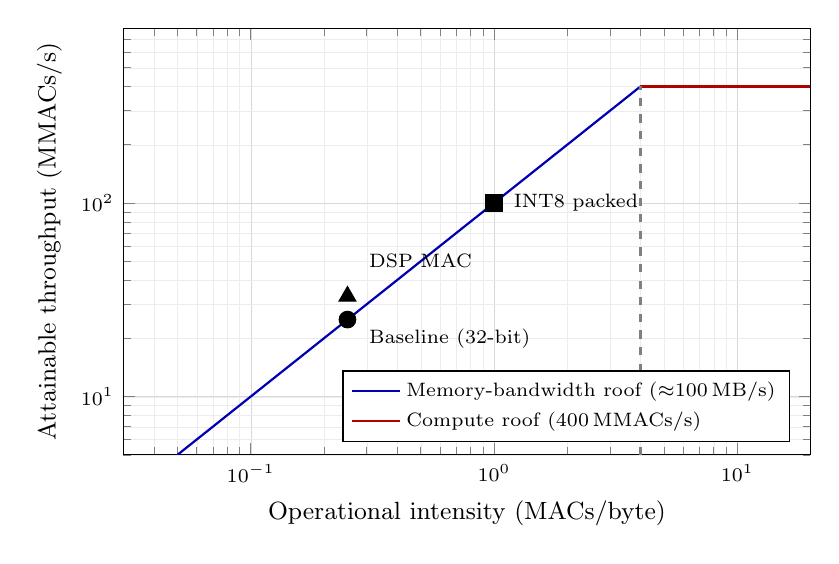
\begin{tikzpicture}
    \begin{axis}[
      width=0.85\linewidth, height=7cm,
      xmode=log, ymode=log,
      xlabel={Operational intensity (MACs/byte)},
      ylabel={Attainable throughput (MMACs/s)},
      xmin=0.03, xmax=20,
      ymin=5, ymax=800,
      grid=both,
      major grid style={line width=.1pt,draw=gray!30},
      minor grid style={line width=.05pt,draw=gray!15},
      legend pos=south east,
      legend cell align={left},
      legend style={font=\scriptsize},
      tick label style={font=\scriptsize},
      label style={font=\small},
    ]
      % Memory roof: throughput = BW * OI; BW = 100 MB/s (one 32-bit read per cycle @ 50 MHz = 200 MB/s; but shared => 100)
      % So throughput (MMACs/s) = 100 * OI (if OI in MACs/byte)
      \addplot[domain=0.03:4, samples=2, thick, blue!70!black] {100*x};
      \addlegendentry{Memory-bandwidth roof ($\approx$100\,MB/s)};

      % Compute roof: 400 MMACs/s peak
      \addplot[domain=4:20, samples=2, thick, red!70!black] {400};
      \addlegendentry{Compute roof (400\,MMACs/s)};

      % Connector at the knee (x=4)
      \addplot[domain=4:4, samples=2, thick, dashed, gray] coordinates {(4,5)(4,400)};

      % Baseline point: OI ~ 0.25, throughput limited to 25 MMACs/s
      \addplot[only marks, mark=*, mark size=3pt, black] coordinates {(0.25,25)};
      \node[anchor=west, font=\scriptsize] at (axis cs:0.28,20) {Baseline (32-bit)};

      % DSP MAC point: same OI (memory unchanged), slightly better arithmetic
      \addplot[only marks, mark=triangle*, mark size=3.5pt, black] coordinates {(0.25,33)};
      \node[anchor=west, font=\scriptsize] at (axis cs:0.28,50) {DSP MAC};

      % INT8 point: OI ~ 1.0 (4x more operands per byte), throughput ~100 MMACs/s
      \addplot[only marks, mark=square*, mark size=3pt, black] coordinates {(1.0,100)};
      \node[anchor=west, font=\scriptsize] at (axis cs:1.1,100) {INT8 packed};
    \end{axis}
  \end{tikzpicture}
  \caption{Roofline interpretation of the three accelerator stages on the
           Cyclone~V platform. The baseline and DSP-enhanced designs sit on
           the memory-bandwidth roof: arithmetic throughput is capped by
           operand fetch, so widening the MAC array yields only a small gain.
           INT8 packing raises the operational intensity by a factor of four
           (four operands per 32-bit word), shifting the design rightward and
           upward along the bandwidth roof towards the compute-bound region.}
  \label{fig:roofline}
\end{figure}
